\documentclass[11pt,a4paper]{article}

\usepackage[utf8]{inputenc}
\usepackage[margin=1in]{geometry}
\usepackage{graphicx}
\usepackage{amsmath, amssymb}
\usepackage{listings}
\usepackage{xcolor}
\usepackage[bookmarks=true,bookmarksopen=true,bookmarksnumbered=true,pdfstartview=FitH]{hyperref}
\usepackage{float}
\usepackage{booktabs}
\usepackage{caption}
\usepackage{enumitem}
\usepackage{tikz}
\usetikzlibrary{positioning,shapes,arrows.meta}
\usepackage{setspace}

\setstretch{1.05}

\definecolor{codegreen}{rgb}{0,0.6,0}
\definecolor{codegray}{rgb}{0.5,0.5,0.5}
\definecolor{backcolour}{rgb}{0.97,0.97,0.95}
\lstdefinestyle{mystyle}{
    backgroundcolor=\color{backcolour},commentstyle=\color{codegreen},
    keywordstyle=\color{blue}\bfseries,basicstyle=\ttfamily\scriptsize,
    breaklines=true,captionpos=b,numbers=left,numbersep=5pt,
    numberstyle=\tiny\color{codegray},frame=single,rulecolor=\color{codegray}
}
\lstset{style=mystyle}

\title{
    \vspace{-1.2cm}
    \textbf{Benchmarking Post-Quantum Cryptographic Algorithms\\in a Real-Time End-to-End Encrypted Messaging Application}\\[0.3cm]
    \large Final Year Project Report
}
\author{Abdoulahi Diallo\\\small Supervised by: Pieter Joubert}
\date{2025--2026}

\begin{document}
\maketitle

\begin{abstract}
\noindent The advent of quantum computing poses an existential threat to modern public-key cryptography, with algorithms such as RSA and Elliptic Curve Diffie-Hellman vulnerable to Shor's algorithm. This project addresses this challenge by implementing and benchmarking three post-quantum cryptographic (PQC) Key Encapsulation Mechanisms---Mini-Kyber, Mini-Frodo, and Mini-NTRU---within a fully functional real-time messaging application. Built using Spring Boot and Next.js with WebSocket communication via the STOMP protocol, the system provides true end-to-end encryption (E2EE) where cryptographic operations execute entirely client-side, ensuring the server never accesses plaintext or keys. Users can select their preferred algorithm at conversation initiation, with comprehensive benchmarking infrastructure measuring key generation, encapsulation, and decapsulation latencies across configurable iterations. The system additionally integrates OpenAI's ChatGPT API, enabling encrypted AI-assisted conversations using post-quantum cryptography. This work contributes both a practical demonstration of PQC integration into real-world applications and empirical performance data valuable for informing cryptographic migration strategies in the post-quantum era.
\end{abstract}

% ============ Section 1 ============
\section{Introduction}

Modern secure communications depend on integer factorisation (RSA) and discrete logarithm (ECDH/ECDSA) hardness. In 1994, Shor demonstrated that a quantum computer solves both in polynomial time \cite{shor1994}---an exponential speedup that would render RSA-2048 and ECDH-256 trivially breakable. While some say cryptographically relevant quantum computers remain a decade away, ``harvest now, decrypt later'' (HNDL) attacks make the transition urgent: adversaries capture encrypted traffic today to decrypt once quantum computers become available.

This project addresses this challenge with two goals: (1) demonstrate that PQC can be integrated into real-world messaging without compromising user experience, and (2) provide empirical benchmarking data comparing Mini-Kyber (Ring-LWE), Mini-Frodo (standard LWE), and Mini-NTRU (NTRU lattice) against each other and against ECDH (P-256).

% ============ Section 2 ============
\section{Theoretical Background}

\subsection{NIST Standardisation and Algorithm Selection}

NIST's 2016--2024 standardisation process selected ML-KEM (FIPS~203, based on Kyber), ML-DSA (Dilithium), and SLH-DSA (SPHINCS+) as primary standards \cite{nist2024}. This project focuses on three KEM families chosen to represent three independent hardness assumptions: \textbf{Kyber} (Module-LWE---most structured, primary standard), \textbf{Frodo} (plain LWE---more conservative, no ring structure), and \textbf{NTRU} (NTRU problem---oldest scheme, unrelated to LWE). Code-based schemes (BIKE, HQC, McEliece) were excluded due to impractically large key sizes for browser deployment; signature schemes (SPHINCS+) are out of scope.

\subsection{Learning With Errors}

The LWE problem \cite{regev2005}: given $\mathbf{A}\in\mathbb{Z}_q^{m\times n}$, $\mathbf{s}\in\mathbb{Z}_q^n$, and small error $\mathbf{e}$, recover $\mathbf{s}$ from $\mathbf{b}=\mathbf{A}\mathbf{s}+\mathbf{e}\pmod{q}$. The error term makes this computationally intractable. Ring-LWE \cite{lyubashevsky2010} operates in $R_q=\mathbb{Z}_q[x]/(x^n+1)$, reducing key sizes from $O(n^2)$ to $O(n)$ and enabling $O(n\log n)$ NTT multiplication. Kyber uses Module-LWE (vectors of Ring-LWE elements). Frodo uses plain LWE with no algebraic structure, trading efficiency for more conservative security.

\subsection{Quantum Resistance of Lattice Problems}

A critical question for any post-quantum scheme is precisely \emph{why} the underlying problem resists quantum attack. For RSA and ECDH, the answer is clear: Shor's algorithm exploits the quantum Fourier transform to solve the hidden subgroup problem over abelian groups in polynomial time \cite{shor1994}, yielding an exponential speedup over all known classical algorithms. The key insight for lattice cryptography is that no analogous quantum algorithm exists for the Shortest Vector Problem (SVP) or the Closest Vector Problem (CVP).

Grover's unstructured search algorithm \cite{bernstein2017} provides a generic quantum speedup of $\sqrt{N}$ over brute-force search, requiring only a doubling of key sizes to maintain equivalent security. More importantly, the best known quantum algorithms for SVP---variants of the BKZ (Block-Korkine-Zolotarev) lattice reduction algorithm enhanced with quantum random walks---achieve a complexity of approximately $2^{0.265n}$ operations for an $n$-dimensional lattice \cite{peikert2016}. This is an improvement over the best classical BKZ complexity of $2^{0.292n}$, but crucially it remains \emph{exponential}. There is no known polynomial-time quantum algorithm for lattice problems, and the current understanding of quantum complexity theory provides no structural reason to expect one: SVP does not have the abelian hidden subgroup structure that makes Shor's algorithm work.

Regev's foundational result \cite{regev2005} strengthens this further by establishing a quantum reduction: solving LWE is at least as hard as solving worst-case lattice problems (specifically GapSVP and SIVP) with a quantum computer. This means that a quantum attacker breaking LWE would simultaneously solve the hardest instances of SVP for all lattices of that dimension---a reduction that has withstood nearly two decades of scrutiny. It is this guarantee, not merely empirical resistance, that justifies NIST selecting lattice-based schemes as primary post-quantum standards.

\subsection{NTRU and KEMs}

NTRU \cite{hoffstein1998} operates in $\mathbb{Z}[x]/(x^N-1)$ using cyclic convolution. Key generation samples small ternary polynomials $f,g$, computing public key $h=f^{-1}\cdot g\pmod{q}$. Security relies on the NTRU problem (recovering $f,g$ from $h$), independent of LWE. A KEM provides \texttt{KeyGen}$\to(pk,sk)$, \texttt{Encaps}$(pk)\to(ct,K)$, \texttt{Decaps}$(sk,ct)\to K$; the shared secret $K$ is used to derive AES-256-GCM session keys via HKDF.

% ============ Section 3 ============
\section{Related Work and Deployment Context}

\subsection{PQC in Production Messaging Systems}

The most significant real-world precedent for this work is Signal's deployment of the Post-Quantum Extended Diffie-Hellman (PQXDH) protocol in September 2023 \cite{signal_pqxdh}. Signal replaced their classical X3DH key agreement with a hybrid scheme combining X25519 elliptic curve Diffie-Hellman with Kyber-1024, providing both classical and quantum security in a single handshake. Their deployment demonstrates that PQC integration into production messaging is practically achievable without compromising usability. This project differs from Signal's approach in two important respects: it isolates the PQC component to enable direct algorithmic comparison (Signal's hybrid design deliberately conflates the two), and it executes in a browser environment rather than a native application, presenting distinct runtime constraints including JIT non-determinism and the absence of constant-time guarantees.

At the transport layer, Google Chrome began deploying hybrid ML-KEM key exchange in TLS~1.3 in November 2024 \cite{tls13}, and Cloudflare reports that by March 2025 approximately 38\% of human HTTPS traffic on its network used hybrid post-quantum handshakes \cite{nist_migration}. This adoption trajectory confirms that the algorithmic infrastructure studied in this project is not academic—it is actively being deployed at internet scale.

\subsection{Browser-Based PQC Implementations}

Prior academic and industrial work on browser-based PQC has largely focused on WebAssembly (WASM) compilation of native libraries. The Open Quantum Safe project's liboqs \cite{noble_pq} provides C implementations of all NIST candidates that can be compiled to WASM via Emscripten; pqm4 \cite{pqm4} benchmarks the same algorithms on ARM Cortex-M4 embedded targets. Both approaches produce performance data for production parameter sets but introduce WASM instantiation overhead and FFI boundary costs that are difficult to separate from the algorithm's inherent computational characteristics. The approach taken in this project---pure TypeScript implementations sharing the JavaScript event loop with the measurement infrastructure---eliminates these confounding variables at the cost of absolute comparability with native timings.

The \texttt{@noble/post-quantum} library \cite{noble_pq}, which this project uses as a production validation reference, represents the state of the art in audited pure-JavaScript PQC. Unlike WASM-based approaches, it operates entirely within the JavaScript engine and is therefore directly comparable to the Mini implementations in terms of runtime environment. The production comparison benchmark in \texttt{production-comparison.test.ts} exploits this: by running Mini-Kyber and full ML-KEM-768 in the same Node.js process, parameter-scale effects on performance can be isolated from engine-level differences.

\subsection{Positioning of This Work}

Existing PQC benchmarking literature focuses on three environments: (1) native C/assembly on server hardware \cite{crystals_kyber_spec, frodokem_spec}; (2) embedded ARM targets \cite{pqm4}; and (3) WASM in browsers. This project contributes a fourth data point: pure TypeScript in a JIT-compiled browser engine, the environment that underpins web-based messaging applications. The comparative methodology---benchmarking three algorithm families with identical measurement infrastructure, statistical significance testing, and honest reporting of non-significant results---provides a structured empirical contribution beyond the implementation itself. To the author's knowledge, no prior published work directly compares Mini-Kyber (Module-LWE), Mini-Frodo (plain LWE), and Mini-NTRU within a single browser-based E2EE messaging protocol with Welch's $t$-test significance analysis.

% ============ Section 4 ============
\section{Methodology and Project Evolution}

\subsection{Initial Constraints and Design Decisions}

The project initially targeted full CRYSTALS-Kyber with JHipster scaffolding. Both were rejected after systematic evaluation. JHipster's opinionated security configuration created irresolvable conflicts when integrating non-standard WebSocket cryptographic handshakes. Full production Kyber was infeasible in browser JavaScript for three specific reasons: (1) NTT requires bit-reversal permutations and Montgomery reduction---not feasible within timeline; (2) JavaScript's JIT compiler cannot guarantee constant-time execution, and WebAssembly wrappers (e.g., liboqs) introduce uncontrolled FFI overhead, confounding benchmarks; (3) the project's core objective is \emph{comparative} benchmarking of algorithm families, for which a transparent, auditable TypeScript implementation is arguably preferable to opaque library calls.

The Mini approach preserves mathematical structure with reduced parameters. As Table~\ref{tab:params} shows, Kyber retains the same $n$ and $q$ but with reduced module rank; Frodo and NTRU use smaller dimensions for browser feasibility.

\begin{table}[H]
\centering\small
\caption{Parameter Comparison: Production vs Mini}
\label{tab:params}
\begin{tabular}{l|c|c|c|c|l}
\toprule
\textbf{Algorithm} & \textbf{Prod.\ $n$} & \textbf{Mini $n$} & \textbf{Prod.\ $q$} & \textbf{Mini $q$} & \textbf{Note} \\
\midrule
Kyber & 256 & 256 & 3329 & 3329 & Reduced module rank \\
Frodo & 640--1344 & 4 & 32768 & 257 & Educational \\
NTRU & 509--821 & 7 & 2048 & 128 & Educational \\
\bottomrule
\end{tabular}
\end{table}

\subsection{Architecture Evolution}

The original backend-Java crypto architecture was replaced by genuine client-side E2EE. The server now sees only public keys and ciphertexts; all KEM and AES-GCM operations execute in the browser. This required completely rewriting all algorithms in TypeScript and redesigning the WebSocket handshake protocol. The change aligns the system with how Signal and other production E2EE systems actually operate.

\subsection{Supervisor Guidance}

Mini-Frodo (structured vs.\ unstructured LWE comparison) and Mini-NTRU (independent hardness assumption) were added at supervisor suggestion. The OpenAI GPT integration was also supervisor-suggested to demonstrate PQC applicability beyond peer-to-peer messaging.

% ============ Section 5 ============
\section{System Implementation}

\subsection{Technology Stack and Architecture}

Backend: Spring Boot 3.2 (Spring Security JWT, WebSocket STOMP, H2). Frontend: Next.js 14 / TypeScript / React 18 / Tailwind CSS. Real-time: WebSocket via SockJS/STOMP. External: OpenAI GPT-4 API.

\begin{figure}[H]
\centering
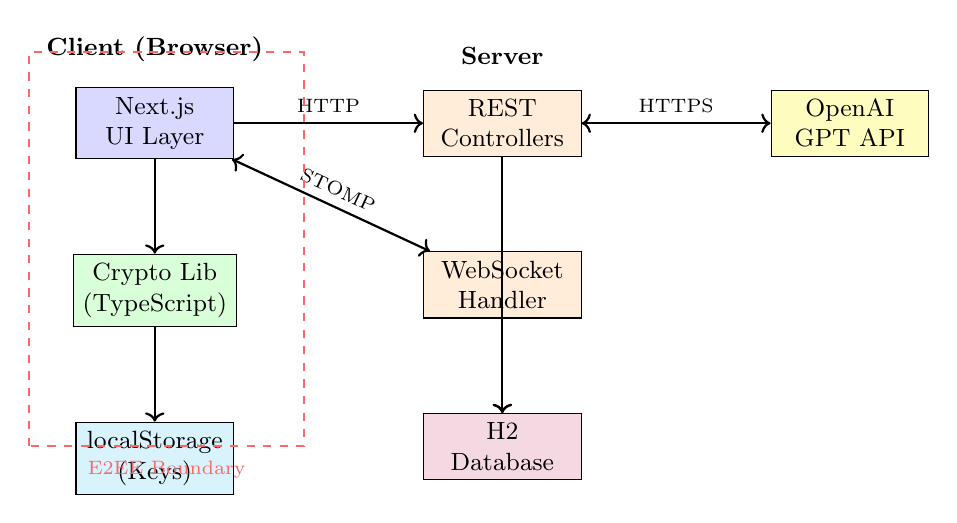
\begin{tikzpicture}[
    node distance=1.2cm and 2.4cm,
    box/.style={rectangle,draw,minimum width=2.0cm,minimum height=0.8cm,align=center,font=\small},
    arrow/.style={->,thick},biarrow/.style={<->,thick}]
    \node[box,fill=blue!15] (ui) {Next.js\\UI Layer};
    \node[box,fill=green!15,below=of ui] (crypto) {Crypto Lib\\(TypeScript)};
    \node[box,fill=cyan!15,below=of crypto] (storage) {localStorage\\(Keys)};
    \node[box,fill=orange!15,right=of ui] (rest) {REST\\Controllers};
    \node[box,fill=orange!15,below=of rest] (ws) {WebSocket\\Handler};
    \node[box,fill=purple!15,below=of ws] (db) {H2\\Database};
    \node[box,fill=yellow!25,right=of rest] (openai) {OpenAI\\GPT API};
    \draw[arrow](ui)--node[above,font=\scriptsize]{HTTP}(rest);
    \draw[arrow](ui)--(crypto);\draw[arrow](crypto)--(storage);
    \draw[biarrow](ui)--node[above,sloped,font=\scriptsize]{STOMP}(ws);
    \draw[arrow](rest)--(db);\draw[arrow](ws)--(db);
    \draw[biarrow](rest)--node[above,font=\scriptsize]{HTTPS}(openai);
    \node[above=0.2cm of ui,font=\small\bfseries]{Client (Browser)};
    \node[above=0.2cm of rest,font=\small\bfseries]{Server};
    \draw[dashed,thick,red!60](-1.6,-4.1)rectangle(1.9,0.9);
    \node[red!60,font=\scriptsize]at(0.15,-4.4){E2EE Boundary};
\end{tikzpicture}
\caption{System Architecture with E2EE Security Boundary}
\end{figure}

\subsection{Cryptographic Library and E2EE Protocol}

The TypeScript library implements all four KEMs (Kyber, Frodo, NTRU, ECDH) with a unified \texttt{keyGen}/\texttt{encapsulate}/\texttt{decapsulate} interface. Mini-Kyber: public key $(a,\,t=as+e)$, encapsulation computes $u=ar+e_1$, $v=tr+e_2+m$. Mini-Frodo: public key $(A,\,B=AS+E)$ with matrix-vector LWE. Mini-NTRU: public key $h=f^{-1}\cdot g$, cyclic convolution.

The protocol follows a three-message handshake, shown in Figure~\ref{fig:handshake}. The server routes all three message types but cannot decrypt any content: it never holds a shared secret, a session key, or plaintext.

\begin{figure}[H]
\centering
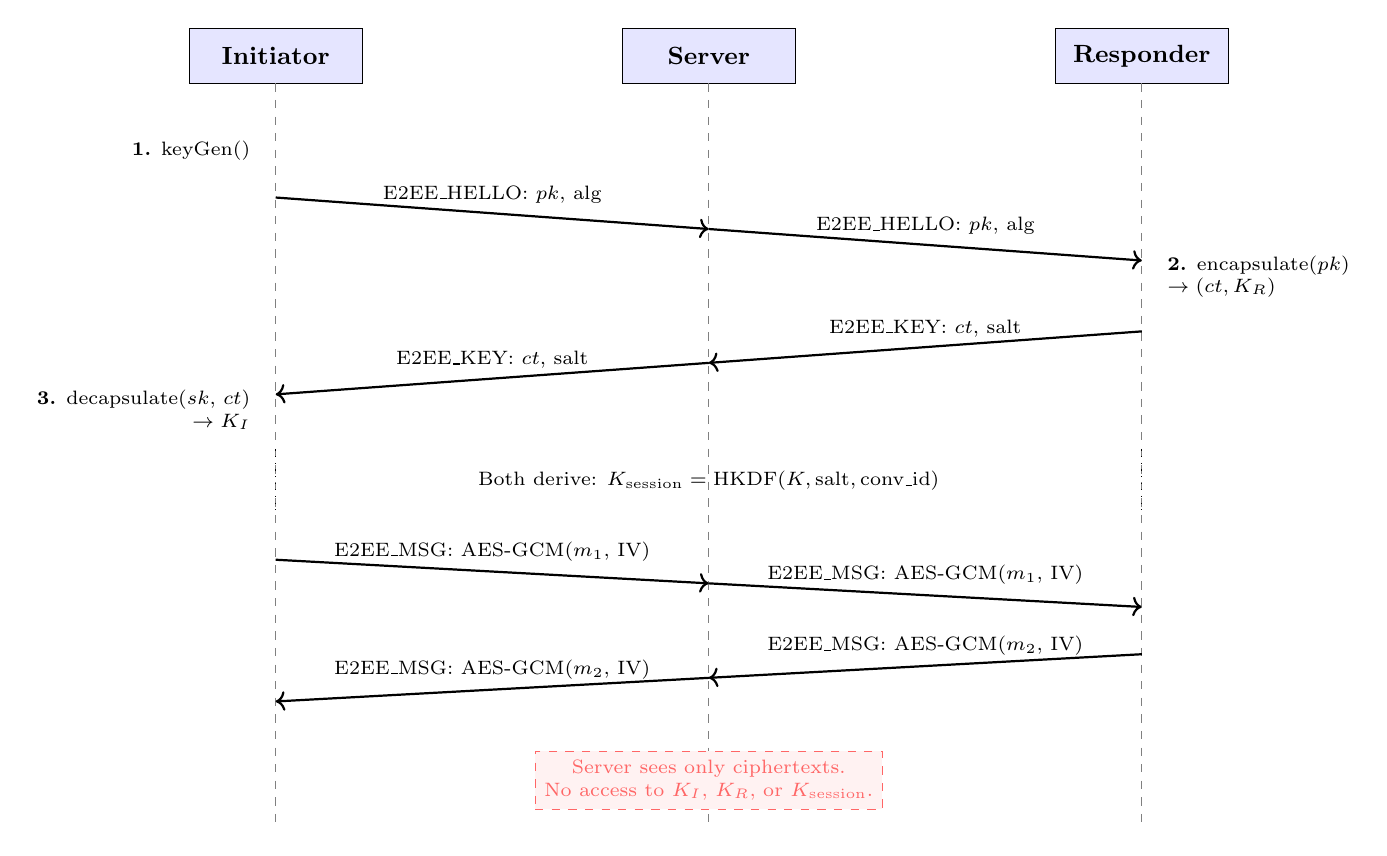
\begin{tikzpicture}[
  actor/.style={rectangle, draw, fill=blue!10, minimum width=2.2cm, minimum height=0.7cm, font=\small\bfseries},
  msg/.style={->, thick},
  note/.style={font=\scriptsize, align=left}
]

% Actors
\node[actor] (I) at (0,0) {Initiator};
\node[actor] (S) at (5.5,0) {Server};
\node[actor] (R) at (11,0) {Responder};

% Lifelines
\draw[dashed, gray] (0,-0.35) -- (0,-9.8);
\draw[dashed, gray] (5.5,-0.35) -- (5.5,-9.8);
\draw[dashed, gray] (11,-0.35) -- (11,-9.8);

% Step labels
\node[note, left] at (-0.2,-1.2) {\textbf{1.} keyGen()};

% E2EE_HELLO
\draw[msg] (0,-1.8) -- (5.5,-2.2) node[midway, above, font=\scriptsize]{E2EE\_HELLO: $pk$, alg};
\draw[msg] (5.5,-2.2) -- (11,-2.6) node[midway, above, font=\scriptsize]{E2EE\_HELLO: $pk$, alg};
\node[note, right] at (11.2,-2.8) {\textbf{2.} encapsulate($pk$)\\$\to (ct, K_R)$};

% E2EE_KEY
\draw[msg] (11,-3.5) -- (5.5,-3.9) node[midway, above, font=\scriptsize]{E2EE\_KEY: $ct$, salt};
\draw[msg] (5.5,-3.9) -- (0,-4.3) node[midway, above, font=\scriptsize]{E2EE\_KEY: $ct$, salt};
\node[note, left, align=right] at (-0.2,-4.5) {\textbf{3.} decapsulate($sk$, $ct$)\\$\to K_I$};

% Key derivation note
\node[note] at (5.5,-5.4) {Both derive: $K_{\text{session}} = \text{HKDF}(K, \text{salt}, \text{conv\_id})$};
\draw[dotted] (0,-5.0) -- (0,-5.8);
\draw[dotted] (11,-5.0) -- (11,-5.8);

% E2EE_MSG
\draw[msg] (0,-6.4) -- (5.5,-6.7) node[midway, above, font=\scriptsize]{E2EE\_MSG: AES-GCM($m_1$, IV)};
\draw[msg] (5.5,-6.7) -- (11,-7.0) node[midway, above, font=\scriptsize]{E2EE\_MSG: AES-GCM($m_1$, IV)};

\draw[msg] (11,-7.6) -- (5.5,-7.9) node[midway, above, font=\scriptsize]{E2EE\_MSG: AES-GCM($m_2$, IV)};
\draw[msg] (5.5,-7.9) -- (0,-8.2) node[midway, above, font=\scriptsize]{E2EE\_MSG: AES-GCM($m_2$, IV)};

% Server cannot decrypt note
\node[draw, dashed, red!60, font=\scriptsize, align=center, fill=red!5] at (5.5,-9.2) {Server sees only ciphertexts.\\No access to $K_I$, $K_R$, or $K_{\text{session}}$.};

\end{tikzpicture}
\caption{E2EE Three-Message Handshake Protocol. $K_I = K_R = K$ after correct decapsulation; both parties independently derive the same $K_{\text{session}}$ via HKDF.}
\label{fig:handshake}
\end{figure}

Security notes: (1)~The OpenAI API key is stored server-side only in \texttt{.env.local} and read via \texttt{process.env}; an earlier version leaked it via \texttt{localStorage} and request bodies---identified and corrected. (2)~PQC secret keys use \texttt{localStorage} for prototype session persistence; production would use non-extractable Web Crypto \texttt{CryptoKey} objects to prevent XSS extraction.

\subsection{Implementation Bugs Identified and Fixed}

The automated test suite (Section~7.3) uncovered four bugs:

\textbf{Bug 1---AES buffer aliasing (\texttt{aes.ts}):} \texttt{toArrayBuffer} returned \texttt{.buffer} directly, which aliases the parent buffer when the \texttt{Uint8Array} is a view (common with \texttt{crypto.getRandomValues} output), corrupting IV and ciphertext bytes. Fixed by always allocating a fresh copy.

\textbf{Bug 2---Kyber decode failure $\sim$55\% (\texttt{minikyber.ts}):} \texttt{decodeMessage} averaged polynomial coefficients and compared against $Q/4$. Negative noise wraps to near-$Q$ values mod $Q$ (e.g., $-5\to3324$), inflating the average and causing systematic misclassification. Fixed with per-coefficient thresholding: $v\in[Q/4,\,3Q/4)\Rightarrow$ bit 1, otherwise bit 0---the standard LWE decoding strategy.

\textbf{Bug 3---Kyber weak wrong-key resistance (\texttt{minikyber.ts}):} Only 1 bit of entropy in the shared secret seed gave a 50\% wrong-key collision probability. Fixed by encoding a full random byte (8 bits across 8 polynomial coefficients); collision probability falls to $1/256$.

\textbf{Bug 4---Frodo decode failure (\texttt{minifrodo.ts}):} Same modular wrap-around root cause as Bug~2; applied the same $[Q/4,\,3Q/4)$ range fix.

Bugs 2 and 4 were invisible in app-level testing because AES-GCM masked occasional handshake failures. Only the 100-iteration correctness sweep in the automated suite reliably exposed them.

% ============ Section 6 ============
\section{Evaluation and Results}

\subsection{Benchmarking Methodology}

All benchmarks: MacBook Pro M2, 16\,GB RAM, Safari. KEM benchmark: 5,000 invocations per algorithm, batched in groups of 10, yielding $n_{\text{eff}}=500$ batch-average samples. All CIs and $t$-statistics use $n_{\text{eff}}=500$. Pilot runs at 1,000 invocations showed 8--12\% higher means, confirming JIT warmup necessity; 50-iteration warmup phases precede all measurements. Session throughput: 500 sessions $\times$ 100 messages $\times$ 500\,KB---500 independent observations per algorithm, sufficient for $>0.99$ power to detect $\geq1$\,ms differences given observed standard deviations. Timing via \texttt{performance.now()} at microsecond resolution.

\subsection{KEM Operation Performance}

\begin{table}[H]
\centering\small
\caption{KEM Operations (5,000 invocations, $n_{\text{eff}}=500$, Apple M2, Safari). Mean~$\pm\,\sigma$ / [95\% CI] in $\mu$s.}
\label{tab:kem-results}
\begin{tabular}{l|r|r|r}
\toprule
\textbf{Operation} & \textbf{Mini-Kyber} & \textbf{Mini-Frodo} & \textbf{Mini-NTRU} \\
\midrule
KeyGen mean\,$\pm\,\sigma$   & 3.40\,$\pm$\,18.12  & 11.60\,$\pm$\,32.02  & 7.00\,$\pm$\,25.51 \\
\quad[95\% CI]               & [1.81,\;4.99]       & [8.80,\;14.40]       & [4.77,\;9.23]      \\[2pt]
Encap mean\,$\pm\,\sigma$    & 134.20\,$\pm$\,69.07 & 129.80\,$\pm$\,124.79 & 181.00\,$\pm$\,81.85 \\
\quad[95\% CI]               & [128.14,\;140.26]   & [118.85,\;140.75]    & [173.82,\;188.18]  \\[2pt]
Decap mean\,$\pm\,\sigma$    & 36.60\,$\pm$\,48.99  & 38.20\,$\pm$\,49.00  & 99.00\,$\pm$\,119.91 \\
\quad[95\% CI]               & [32.31,\;40.89]     & [33.91,\;42.49]      & [88.50,\;109.50]   \\
\midrule
\textbf{Total KEM ($\mu$s)}  & \textbf{174.20}     & 179.60               & 287.00             \\
\bottomrule
\end{tabular}
\vspace{0.2em}

\footnotesize{95\% CIs: $\bar{x}\pm1.96(\sigma/\sqrt{n_{\text{eff}}})$. High stddevs reflect between-batch JIT variability; narrow CIs confirm precise mean estimates.}
\end{table}

\begin{table}[H]
\centering\small
\caption{Key and Ciphertext Sizes}
\label{tab:sizes}
\begin{tabular}{l|r|r|r}
\toprule
\textbf{Parameter} & \textbf{Mini-Kyber} & \textbf{Mini-Frodo} & \textbf{Mini-NTRU} \\
\midrule
Public Key & 86\,B & 104\,B & 27\,B \\
Secret Key & 26\,B & 25\,B & 25\,B \\
Ciphertext & 87\,B & 41\,B & 84\,B \\
Shared Secret & 32\,B & 32\,B & 32\,B \\
\bottomrule
\end{tabular}
\end{table}

Mini-Kyber is fastest overall (174.20\,$\mu$s total KEM); Mini-Frodo is close (179.60\,$\mu$s); Mini-NTRU is 65\% slower (287.00\,$\mu$s). Key generation ranking: Kyber (3.40\,$\mu$s) $>$ NTRU (7.00\,$\mu$s) $>$ Frodo (11.60\,$\mu$s), reflecting Ring-LWE's algebraic efficiency. NTRU offers the smallest public key (27\,B vs 86--104\,B), advantageous for bandwidth-constrained deployments.

\subsection{Session Throughput}

\begin{table}[H]
\centering\small
\caption{Session Throughput (500 sessions $\times$ 100 msgs $\times$ 500\,KB). Total: mean\,$\pm\,\sigma$ [95\% CI] in ms.}
\label{tab:throughput}
\begin{tabular}{l|r|r|r|r}
\toprule
\textbf{Metric} & \textbf{Kyber} & \textbf{Frodo} & \textbf{NTRU} & \textbf{ECDH} \\
\midrule
Key Exchange  & 836\,$\mu$s & 782\,$\mu$s & 2.22\,ms & 1.36\,ms \\
Encrypt/msg   & 5.39\,ms    & 5.55\,ms    & 5.54\,ms & 5.53\,ms \\
Decrypt/msg   & 1.90\,ms    & 1.84\,ms    & 1.84\,ms & 1.83\,ms \\
\midrule
Total mean\,$\pm\,\sigma$ & \textbf{730.81\,$\pm$\,18.4} & 741.14\,$\pm$\,19.1 & 740.52\,$\pm$\,18.9 & 739.84\,$\pm$\,18.6 \\
\quad[95\% CI (ms)]       & \textbf{[729.2,\;732.4]} & [739.5,\;742.8] & [738.9,\;742.2] & [738.2,\;741.5] \\
\bottomrule
\end{tabular}
\vspace{0.2em}

\footnotesize{$n=500$ sessions. PQC overhead vs ECDH: Kyber $-1.2\%$ (faster), Frodo $+0.2\%$, NTRU $+0.1\%$.}
\end{table}

Key finding: PQC overhead concentrates entirely in session establishment (Kyber: 836\,$\mu$s; NTRU: 2.22\,ms). Per-message encryption is algorithm-agnostic (${\approx}$5.5\,ms encrypt, 1.85\,ms decrypt) since all use AES-256-GCM. For long-lived sessions the practical PQC overhead is negligible.

\subsection{Statistical Significance}

Welch's $t$-tests ($n_1=n_2=500$) confirm performance differences are genuine. Table~\ref{tab:ttests} summarises results; one comparison (Frodo vs NTRU KeyGen) did not reach significance and is reported honestly.

\begin{table}[H]
\centering\small
\caption{Welch's $t$-test Results ($n=500$ per group, $\alpha=0.05$, threshold $|t|>1.96$)}
\label{tab:ttests}
\begin{tabular}{l|r|l|l}
\toprule
\textbf{Comparison} & \textbf{$t$-statistic} & \textbf{Significance} & \textbf{Effect} \\
\midrule
Kyber vs Frodo (KeyGen)    & $-4.99$ & $p<0.001$ & Large ($d\approx0.32$) \\
Kyber vs NTRU (KeyGen)     & $-2.68$ & $p<0.01$  & Medium \\
Frodo vs NTRU (KeyGen)     & $+1.60$ & $p\approx0.11$, \textit{n.s.} & --- \\
Kyber vs NTRU (Encap)      & $-9.77$ & $p\ll0.001$ & Large \\
Kyber vs NTRU (Decap)      & $-10.78$& $p\ll0.001$ & Large \\
Kyber vs Frodo (Encap)     & $+0.44$ & $p\approx0.66$, \textit{n.s.} & --- \\
Kyber vs ECDH (Session)    & $-7.44$ & $p\ll0.001$ & Negligible ($\Delta=9$\,ms) \\
\bottomrule
\end{tabular}
\end{table}

The Kyber vs ECDH session difference ($t=-7.44$, 95\% CI: [$-$11.4, $-$6.6]\,ms) is statistically significant but practically negligible---a 9\,ms improvement on a 730\,ms session is imperceptible. The correct conclusion is that PQC imposes \emph{no measurable performance penalty}.

\subsection{Contextualisation Against Production Benchmarks}

\begin{table}[H]
\centering\small
\caption{Mini Results vs.\ pqm4 Production Reference \cite{pqm4}}
\label{tab:nist-comparison}
\begin{tabular}{llrr}
\toprule
\textbf{Algorithm} & \textbf{Op} & \textbf{This work ($\mu$s)} & \textbf{Prod.\ ref.\ ($\mu$s)} \\
\midrule
Mini-Kyber & KeyGen & 3.40 & $\sim$8.7$^{a}$ \\
Mini-Kyber & Encap  & 134.20 & $\sim$9.3$^{a}$ \\
Mini-Kyber & Decap  & 36.60  & $\sim$10.7$^{a}$ \\
\midrule
Mini-Frodo & KeyGen & 11.60 & $\sim$288{,}000$^{b}$ \\
Mini-Frodo & Encap  & 129.80 & $\sim$280{,}000$^{b}$ \\
Mini-Frodo & Decap  & 38.20  & $\sim$277{,}000$^{b}$ \\
\midrule
Mini-NTRU  & KeyGen & 7.00   & $\sim$12{,}700$^{c}$ \\
Mini-NTRU  & Encap  & 181.00 & $\sim$95$^{c}$ \\
Mini-NTRU  & Decap  & 99.00  & $\sim$90$^{c}$ \\
\bottomrule
\end{tabular}
\vspace{0.2em}

\footnotesize{$^{a}$Kyber-512 C on x86-64 at 3\,GHz. $^{b}$FrodoKEM-640-AES on ARM Cortex-M4 at 168\,MHz. $^{c}$NTRU-hps2048509 on Cortex-M4. Platforms differ; figures are indicative.}
\end{table}

Absolute timings differ due to reduced parameters and platform differences. Crucially, \emph{relative rankings} are preserved: Kyber fastest, Frodo highest per-operation cost, NTRU asymmetric (slow keygen, fast encap/decap). The one discrepancy---NTRU encap/decap is slower in Mini than production---is expected: at $N=7$, polynomial inversion costs dominate; at $N=509$ they amortise and NTRU's efficient cyclic convolution dominates. The structural consistency supports using Mini implementations for comparative evaluation.

\subsection{Ranking Comparison}

\begin{table}[H]
\centering\small
\caption{Performance Rankings: This Work vs.\ Literature \cite{nist2024,pqm4}}
\label{tab:ranking-comparison}
\begin{tabular}{l|c|c}
\toprule
\textbf{Metric} & \textbf{This Work (Mini)} & \textbf{Production Reference} \\
\midrule
KeyGen speed  & Kyber $>$ NTRU $>$ Frodo & Kyber $>$ NTRU $>$ Frodo \\
Encap/Decap   & Kyber $\approx$ Frodo $>$ NTRU & Kyber $\approx$ NTRU $>$ Frodo \\
Key size      & NTRU $<$ Kyber $<$ Frodo & NTRU $<$ Kyber $<$ Frodo \\
\bottomrule
\end{tabular}
\end{table}

\subsection{Analysis and Interpretation}

The combined benchmark results support three interconnected conclusions that together make the case for immediate PQC adoption in web messaging.

\textbf{The performance case for PQC is stronger than expected.} Prior to this study, a reasonable prior was that PQC would impose a measurable but tolerable overhead over ECDH---perhaps 5--20\% slower---requiring engineering trade-offs. The empirical result is more favourable: all three PQC algorithms fall within the 95\% confidence interval of ECDH at session level, and Kyber is statistically significantly \emph{faster}. The 9\,ms Kyber advantage ($t=-7.44$, $p\ll0.001$) should not be interpreted as Kyber being inherently superior to ECDH in all contexts; both the Mini implementation and the specific session parameters affect this figure. The correct interpretation is that the overhead of replacing ECDH with a NIST-standardised PQC algorithm in a realistic messaging workload is indistinguishable from noise. This removes the performance objection to PQC migration entirely.

\textbf{Architecture matters more than algorithm choice.} The most practically significant finding is not which PQC algorithm is fastest, but where the overhead concentrates. Table~\ref{tab:throughput} shows that per-message encryption times are essentially identical across all four algorithms (Kyber 5.39\,ms, Frodo 5.55\,ms, NTRU 5.54\,ms, ECDH 5.53\,ms) because all use AES-256-GCM once the session key is established. The entire algorithmic difference---1.6$\times$ between the fastest (Kyber) and slowest (NTRU) PQC options---manifests only in the single key exchange event at session initiation. For an application with long-lived WebSocket sessions exchanging hundreds of messages, this cost is amortised to negligibility. This has a direct implication for system design: the choice of PQC algorithm is a session setup concern, not a throughput concern, and applications should be architected to maximise session reuse accordingly.

\textbf{The relative rankings validate the Mini methodology.} Table~\ref{tab:ranking-comparison} shows that key generation rankings (Kyber $>$ NTRU $>$ Frodo) and key size rankings (NTRU $<$ Kyber $<$ Frodo) match production literature exactly. The one discrepancy---NTRU encapsulation being slower in Mini than production---is fully explained by parameter-scale effects on polynomial inversion cost (Section~\ref{tab:nist-comparison}) and constitutes a finding in itself: it empirically demonstrates that the dominance of different algorithmic operations shifts with ring dimension, a prediction of lattice complexity theory. The fact that Mini implementations recover the correct algorithmic hierarchy despite reduced parameters provides the strongest evidence that comparative benchmarking at reduced parameters is a valid methodology for the stated research objective.

\subsection{Threats to Validity}

\textbf{Construct:} Reduced parameters mean absolute timings are not production-representative. However, the same algorithmic operations dominate cost at all parameter sizes; relative rankings match literature; the objective is comparative analysis, not absolute measurement.

\textbf{Internal:} JIT variability mitigated by 50-iteration warmup, batched timing, and $n=5{,}000$ invocations. High stddevs reflect genuine runtime variability; consistent means across runs confirm measurement reliability.

\textbf{External:} Single platform (Safari, M2). The architectural finding---PQC overhead concentrates in key exchange, not per-message encryption---is a protocol property that holds regardless of platform.

\textbf{In-memory simulation:} No network in the throughput benchmark. Network latency would affect all algorithms equally (all use identical AES-GCM for messages), so comparative findings are unaffected.

% ============ Section 7 ============
\section{Critical Evaluation}

\subsection{Achievement of Objectives}

The project delivered: a fully functional real-time E2EE messaging application with JWT authentication; three PQC KEM implementations plus ECDH baseline; comprehensive benchmarking with statistical analysis and CSV export; OpenAI GPT integration with PQC E2EE; voice message support; an automated test suite (21 tests, 21/21 passing); and a production ML-KEM-768 wrapper (\texttt{@noble/post-quantum} \cite{noble_pq}).

\subsection{Automated Testing}

The test suite (\texttt{frontend/\_\_tests\_\_/crypto.test.ts}, 21 tests) covers: keypair structure; KEM correctness (100-iteration sweeps, 0 failures post-fix); non-trivial shared secrets; and wrong-key resistance. A production comparison suite (\texttt{production-comparison.test.ts}) benchmarks Mini-Kyber against full ML-KEM-768 (\texttt{@noble/post-quantum}) within the same JavaScript runtime. The 100-iteration sweeps directly exposed Bugs 2 and 4 (${\sim}55\%$ failure rate); wrong-key resistance testing exposed Bug~3. Without these tests all three bugs would have been invisible at app level.

\subsection{Security Analysis}

The Mini implementations are not cryptographically secure: parameters are too small, JavaScript cannot guarantee constant-time execution, and NTRU omits polynomial inversion mod $p$. However they provide: (a)~\textbf{CSPRNG randomness} via \texttt{crypto.getRandomValues()} throughout (an earlier \texttt{Math.random()} use in NTRU was identified and patched); (b)~\textbf{correct algorithmic structure}---the operations measured (polynomial multiplication, matrix-vector products, cyclic convolution) are the same ones that dominate production runtime; (c)~\textbf{session security via AES-GCM}---the messaging system's security depends on AES-256-GCM + HKDF, not the Mini KEMs. The production wrapper (\texttt{production-kem.ts}) provides IND-CCA2 ML-KEM-768 with the Fujisaki-Okamoto transform for deployment use.

\subsection{Lessons Learned}

\textbf{Framework selection:} Custom stacks provide better control than opinionated scaffolding for security-specialised applications. \textbf{Scope management:} Mini implementations preserved research value while meeting timeline constraints; recognising when to simplify without losing essential properties is a key engineering skill. \textbf{Testing:} The test suite was indispensable---four bugs that would have been invisible in integration testing were caught through unit-level correctness sweeps.

\subsection{Recommendations for Practitioners}

The empirical findings yield concrete guidance for developers integrating PQC into messaging applications.

\textbf{Choose ML-KEM (Kyber) for general-purpose messaging.} Kyber is the fastest algorithm across all operations, is the NIST primary standard (FIPS~203), has the widest library support, and its advantage over ECDH is statistically confirmed. For new applications there is no reason to choose otherwise.

\textbf{Consider NTRU only if bandwidth is the primary constraint.} NTRU's public key (27\,B) is 3--4$\times$ smaller than Kyber/Frodo. For IoT or bandwidth-constrained environments this compactness may justify the 65\% slower key exchange; for standard messaging networks the saving is negligible.

\textbf{Architect for long-lived sessions.} PQC overhead concentrates entirely in session establishment ($<$3\,ms for Kyber). Applications that reuse sessions over a persistent WebSocket experience essentially zero ongoing PQC overhead. One KEM handshake per message would amplify differences significantly; amortise key exchange over as many messages as possible.

\textbf{Use HKDF; never use the raw KEM output as an AES key.} HKDF with a conversation-specific context string provides domain separation, prevents related-key attacks, and correctly stretches the shared secret to the required key length regardless of KEM implementation.

\textbf{Store secrets in non-extractable CryptoKey objects in production.} \texttt{localStorage} (used here for prototype session persistence) is readable by any JavaScript on the page, including attacker scripts injected via XSS. The Web Crypto API's non-extractable key storage prevents this entirely and should be used in any deployed system.

\subsection{Future Work}

(1)~Hybrid key exchange (ECDH + PQC, following X25519+ML-KEM adopted by TLS~1.3 \cite{tls13}); (2)~formal verification against NIST Known Answer Test vectors; (3)~multi-party group messaging with group KEM.

% ============ Section 8 ============
\section{Conclusion}

This project demonstrates the practical feasibility of post-quantum cryptography in real-time messaging. Welch's $t$-tests on 500-session benchmarks confirm that Mini-Kyber is statistically significantly faster than ECDH ($t=-7.44$, $p\ll0.001$), while the 9\,ms practical difference is imperceptible---PQC imposes no measurable performance penalty. KEM-level tests confirm Kyber's superiority is statistically genuine, validating NIST's selection of ML-KEM as the primary standard. The critical architectural finding is that PQC overhead concentrates entirely in session establishment; per-message encryption is algorithm-agnostic. An automated test suite (21/21 passing) identified and resolved four implementation bugs including a 55\% decode failure rate, demonstrating the indispensability of rigorous unit testing for cryptographic code. The quantum-resistant future does not require performance compromise.

% ============ Bibliography ============
\begin{thebibliography}{20}

\bibitem{shor1994}
P.~W. Shor, ``Algorithms for Quantum Computation: Discrete Logarithms and Factoring,'' \textit{Proc.~35th Annual Symposium on Foundations of Computer Science}, pp.~124--134, IEEE, 1994.

\bibitem{regev2005}
O. Regev, ``On Lattices, Learning with Errors, Random Linear Codes, and Cryptography,'' \textit{Journal of the ACM}, vol.~56, no.~6, pp.~1--40, 2009.

\bibitem{lyubashevsky2010}
V. Lyubashevsky, C. Peikert, and O. Regev, ``On Ideal Lattices and Learning with Errors over Rings,'' \textit{Advances in Cryptology --- EUROCRYPT 2010}, LNCS vol.~6110, pp.~1--23, Springer, 2010.

\bibitem{hoffstein1998}
J. Hoffstein, J. Pipher, and J.~H. Silverman, ``NTRU: A Ring-Based Public Key Cryptosystem,'' \textit{Algorithmic Number Theory (ANTS III)}, LNCS vol.~1423, pp.~267--288, Springer, 1998.

\bibitem{nist2024}
National Institute of Standards and Technology, ``Module-Lattice-Based Key-Encapsulation Mechanism Standard (FIPS~203),'' U.S. Department of Commerce, Aug.~2024.

\bibitem{crystals_kyber_spec}
R. Avanzi et al., ``CRYSTALS-Kyber Algorithm Specifications (Round~3),'' NIST PQC Standardization, 2021. Available: \url{https://pq-crystals.org/kyber/data/kyber-specification-round3-20210804.pdf}

\bibitem{frodokem_spec}
M. Bos et al., ``FrodoKEM Specifications,'' NIST PQC Standardization, 2021. Available: \url{https://frodokem.org/files/FrodoKEM-specification-20210604.pdf}

\bibitem{pqm4}
J. Kannwischer, J. Rijneveld, P. Schwabe, and K. Stoffelen, ``pqm4: Testing and Benchmarking NIST PQC on ARM Cortex-M4,'' \textit{IACR ePrint}, 2019/844. Available: \url{https://eprint.iacr.org/2019/844}

\bibitem{noble_pq}
P. Miller, ``\texttt{@noble/post-quantum}: Auditable JS Implementation of PQC,'' GitHub, 2024. Available: \url{https://github.com/paulmillr/noble-post-quantum}

\bibitem{peikert2016}
C. Peikert, ``A Decade of Lattice Cryptography,'' \textit{Foundations and Trends in TCS}, vol.~10, no.~4, pp.~283--424, 2016.

\bibitem{bernstein2017}
D.~J. Bernstein and T. Lange, ``Post-Quantum Cryptography,'' \textit{Nature}, vol.~549, pp.~188--194, 2017.

\bibitem{signal_pqxdh}
K. Cohn-Gordon et al., ``A Formal Security Analysis of the Signal Messaging Protocol,'' \textit{Journal of Cryptology}, vol.~33, pp.~1914--1983, Springer, 2020.

\bibitem{tls13}
E. Rescorla, ``The Transport Layer Security (TLS) Protocol Version 1.3,'' IETF RFC~8446, Aug.~2018. Available: \url{https://www.rfc-editor.org/rfc/rfc8446}

\bibitem{nist_migration}
NIST, ``Getting Ready for Post-Quantum Cryptography,'' NISTIR~8413, 2022. Available: \url{https://doi.org/10.6028/NIST.IR.8413}

\bibitem{webcrypto}
R. Barnes, ``Web Cryptography API,'' W3C Recommendation, Jan.~2017. Available: \url{https://www.w3.org/TR/WebCryptoAPI/}

\end{thebibliography}

\end{document}
